\documentclass[11pt, oneside]{article} 
\usepackage{geometry}
\geometry{letterpaper} 
\usepackage{graphicx}
	
\usepackage{amssymb}
\usepackage{amsmath}
\usepackage{parskip}
\usepackage{color}
\usepackage{hyperref}

\graphicspath{{/Users/telliott/Github/precalculus/fig/}}
% \begin{center} \includegraphics [scale=0.4] {gauss3.png} \end{center}

\title{Quadrature}
\date{}

\begin{document}
\maketitle
\Large

Hippocrates of Chios (470-410 BC) was a major figure in Greek geometry.  (Not to be confused with the physician of the same name, from Kos).  Hippocrates focused on quadrature, the process of constructing (with straight-edge and compass) a square with area equal to a given geometric figure, particularly curved figures, called lunes.  Here is one of the first of these---construction of the square equivalent to a given rectangle.
\begin{center} 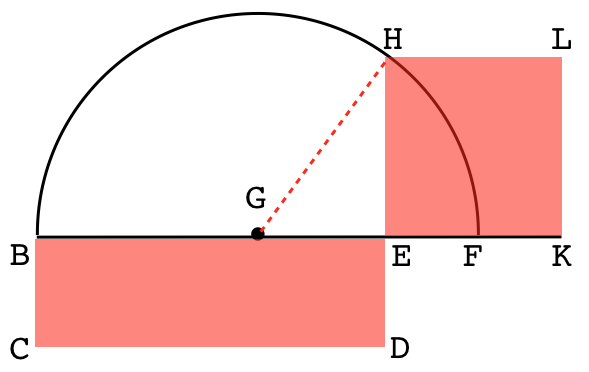
\includegraphics [scale=0.4] {square_rect_1.png} \end{center}

The construction says to:  (i) extend $BE$ horizontally, (ii) mark off the same distance as $DE$ to construct $EF$, (iii) find the midpoint $G$ of $BF$, (iv) draw the half-circle of radius $BG$, (v) extend $DE$ up to meet the circle at $H$, construct the square of side the same length as $EH$.

\begin{center} 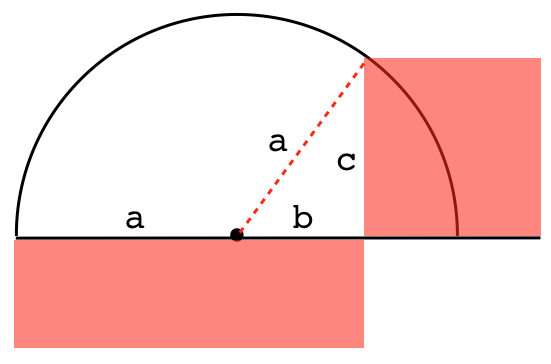
\includegraphics [scale=0.4] {square_rect_2.png} \end{center}

As suggested by the dotted line in the figure, the proof invokes the Pythagorean theorem.  The long side of the rectangle is $a+b$, while its short side is $a - b$, so the area is
\[ A = (a + b)(a - b) = a^2 - b^2 \]
but Pythagoras says that is equal to $c^2$.

$\square$

This is a slight restatement of our proof about the geometric mean.

The side of the square, $c$ is the geometric mean of the sides of the rectangle.
\[ c = \sqrt{(a + b)(a - b)} \]

Hippocrates "squared" rectangles, triangles and polygons.  A lot of his constructions depended on Pythagoras as suggested by this figure:
\begin{center} 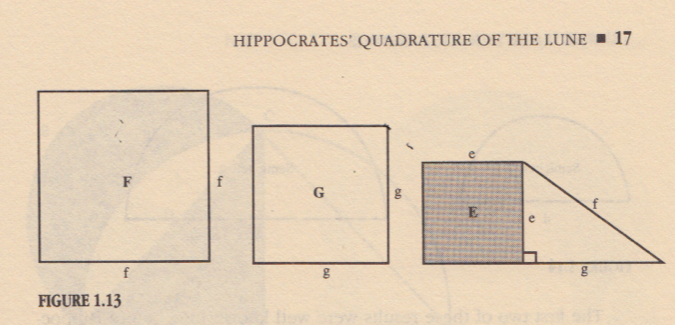
\includegraphics [scale=0.4] {square_addition.png} \end{center}
where two squares resulting from manipulation of part of a polygon need to be subtracted to obtain the final result.

Hippocrates moved on to curves, trying to find squares with area equal to that under or between two curves.  That turns out to be a class of problems where few have solutions (in fact, only five, according to Dunham).  Famously, it is impossible to square the circle.  However, here is one that is possible, it is an example of (the) quadrature of the lune.

\begin{center} 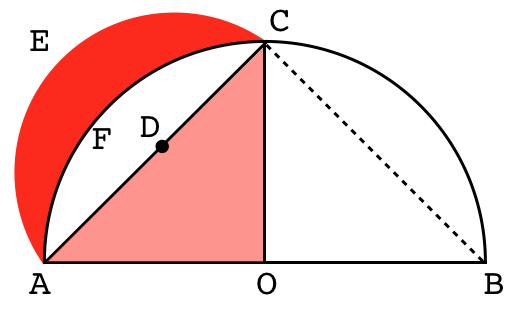
\includegraphics [scale=0.5] {quadrature_lune_2.png} \end{center}
We will prove that the two shaded regions are equal in area.

Consider the smaller semicircle with base $ADC$, which is also the hypotenuse of the right triangle.  Let radius $AD$ be equal to $r$.  Let the large semicircle have radius $AO$ equal to $R$.  Pythagoras tells us that
\[ R^2 + R^2 = (2r)^2 \]
\[ R^2 = 2r^2 \]

Let the area of the triangle be $T$.  (Its value is $R^2/2$ but that's not needed).

The segment of the larger semicircle (white) is the area of the quadrant minus the area of the triangle
\[ \pi \frac{R^2}{4} -  T \]

The area of the red lune is the area of the small semicircle minus the white area
\[ \pi \frac{r^2}{2} - \ [ \ \pi \frac{R^2}{4} -  T \ ] \]
\[ = \pi \frac{r^2}{2} -  \pi \frac{2r^2}{4} + T \]
\[ = T \]
Which is just the area of the triangle.

\begin{center} 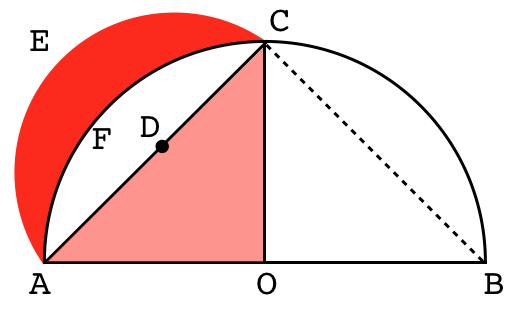
\includegraphics [scale=0.5] {quadrature_lune_2.png} \end{center}

\end{document}